\documentclass[landscape,20pt]{extarticle}
\usepackage[utf8]{inputenc}
\usepackage[T1]{fontenc}
\usepackage[margin=2cm]{geometry}
\usepackage[parfill]{parskip}
\usepackage[pdftex]{graphicx}
%\usepackage[compact]{titlesec}

%\usepackage[sc]{mathpazo}
%\linespread{1.05}         % Palatino needs more leading (space between lines)

\renewcommand{\familydefault}{\sfdefault}
%\renewcommand*\rmdefault{cmfib}

\newcommand*{\TitleFont}{\Huge \bf}

\newcommand*{\TextFont}{\normalsize \it}

\begin{document}
\thispagestyle{empty}
\Large
{\TitleFont Introduction}

\begin{itemize}
\item The value of an Opinion\\
{\TextFont There a lot of different things one can use an opinion for}
\item Analyzing Communication\\
{\TextFont Communication reflects an opinion}
\item Semantic Orientation\\
{\TextFont Detecting if an opinion is negative or positive}
\item Classifying tweets and counting them = opinion?\\
{\TextFont Is there a better way to extract an opinion?}
\item The ``influence'' of a tweet\\
{\TextFont Take followers, retweets and favorites into account!}
\end{itemize}

\clearpage
\thispagestyle{empty}

{\TitleFont System Overview}
\newline
\centerline{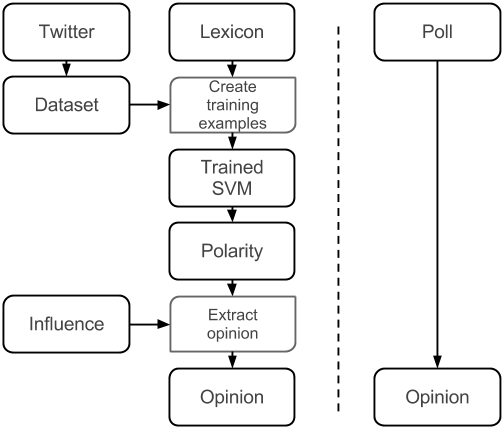
\includegraphics[scale=1]{../img/Overview.png}}

\clearpage
\thispagestyle{empty}

{\TitleFont Method}

\begin{itemize}
\item The opinion of a brand, negative or positive?\\
{\TextFont To keep it simple we measured simply if the opinion was positive or negative}
\item Opinion = position in a range\\
{\TextFont Essentially a score in the [0-100] range where 0 is fully negative}
\item Must still classify tweets using the text alone\\
{\TextFont To use the influence one must know the initial opinion of the brand in the tweet}
\item SVM + Supervised Learning through Lexicons\\
{\TextFont We used a SVM to classify and Lexicons to classify training data for the SVM}
\item Evaluate the Lexicon, the SVM and the final algorithm\\
{\TextFont To make sure the different components yield reasonable results we have to \\evaluate them, we used manual classification and a Poll to evaluate them}
\end{itemize}

\clearpage
\thispagestyle{empty}

{\TitleFont Lexicon \& SVM}

\begin{itemize}
\item We use 7 different lexicons\\
{\TextFont Together they contains 8000 unique words with positive and negative scores.}
\item For each tweet we sum the scores of its words\\
{\TextFont Our pre-processing removes punctuation and lemmatize words for better results.}
\item From this score, we create learning data\\
{\TextFont Positive tweets are the \textit{n} with highest positive score, the same for negative.\\
The neutral tweets are the \textit{n} longest tweets with a score of 0.}
\item The SVM represents the tweets with features\\
{\TextFont These features are the unigrams and bigrams, extracted from the cleaned text.}
\item We make the SVM learn with the generated learning data\\
{\TextFont We then have a classifier for tweets about a company which learn automatically.}
\end{itemize}

\clearpage
\thispagestyle{empty}

{\TitleFont Algorithm}

\clearpage
\thispagestyle{empty}

{\TitleFont Results}
\newline
\small{Manual classification}
\newline
\newline
\newline
\newline
\centerline{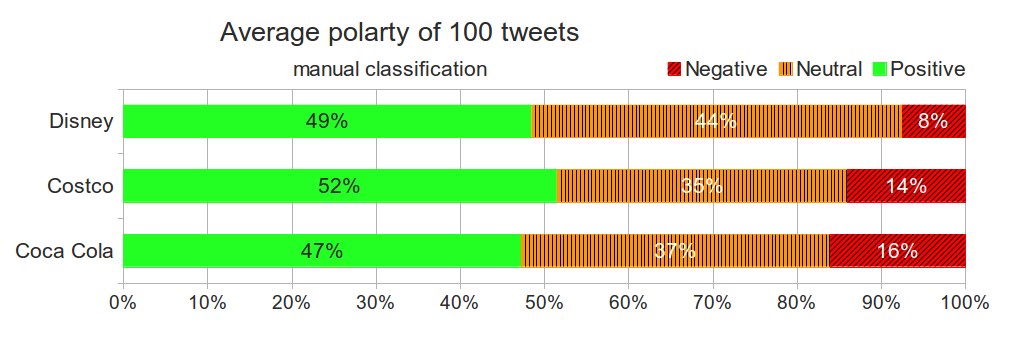
\includegraphics[scale=0.85]{../img/man1.png}}

\clearpage
\thispagestyle{empty}

{\TitleFont Results}
\newline
\small{Polarity scores}
\newline
\centerline{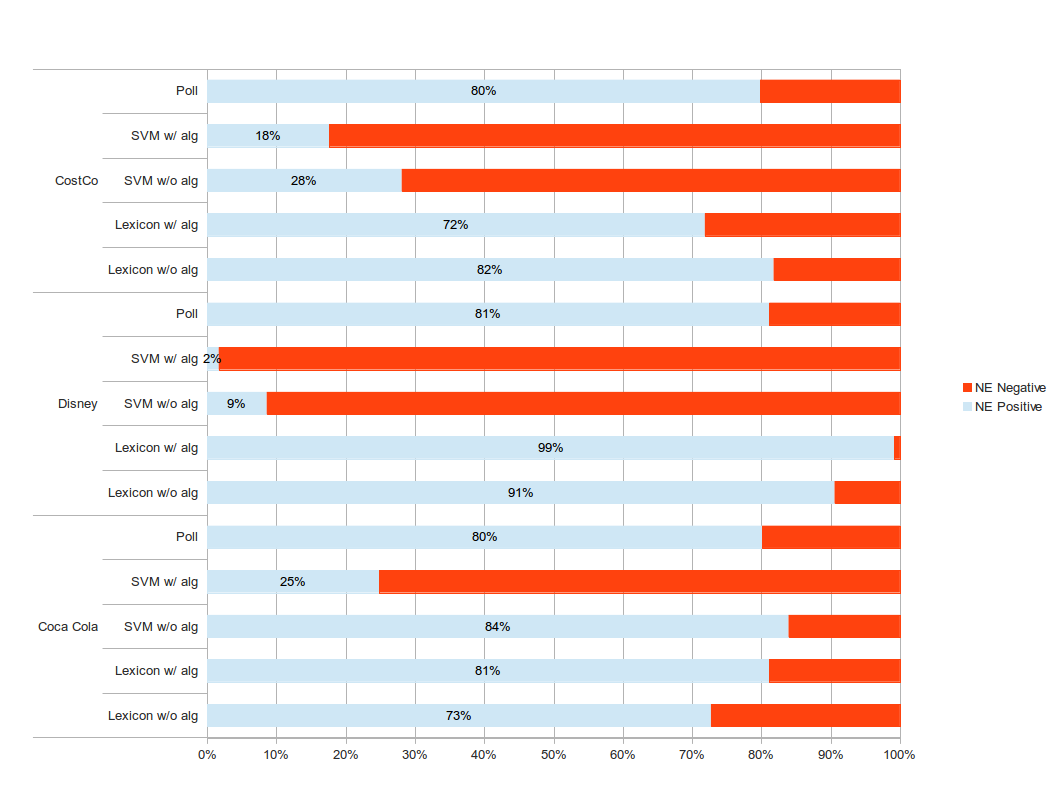
\includegraphics[scale=0.7]{../img/full1.png}}




\clearpage
\thispagestyle{empty}

{\TitleFont Discussion \& Conclusion}
\Large
\begin{itemize}
\item Tweets are notoriously hard to classify\\
{\TextFont Limited word-limit forces people to be very succint}
\item The SVM had major problems\\
{\TextFont More features were needed, less noisy training data}
\item Poll and tweet population and overlapping\\
{\TextFont Filtering on a more local language may improve overlapping}
\item Justifying parameters in the Algorithm\\
{\TextFont More data is needed to get good parameters for the Algorithm}
\item The results hints at improvement\\
{\TextFont It seems like using meta-data may improve an opinion estimation, but better results are required to make a definitive answer}
\end{itemize}

\end{document}
